\documentclass[notes,11pt, aspectratio=169]{beamer}

\usepackage{pgfpages}
% These slides also contain speaker notes. You can print just the slides,
% just the notes, or both, depending on the setting below. Comment out the want
% you want.
\setbeameroption{hide notes} % Only slide
%\setbeameroption{show only notes} % Only notes
%\setbeameroption{show notes on second screen=right} % Both


%% Presentation Themes with a Mini Frame Navigation
\usetheme{Frankfurt}  % a variation of Berlin that is slightly less cluttered by leaving out the subsection* information
\setbeamertemplate{footline}[page number]
%\usetheme[compress]{Berlin}
%\usetheme{Singapore}


%% colors
\usecolortheme{seahorse}
%\usecolortheme{rose}
%\usefonttheme{serif}
%\usefonttheme{professionalfonts}


%% special set
\setbeamertemplate{itemize items}[default]
\setbeamertemplate{enumerate items}[default]
\setbeamerfont{title}{size=\large}
\setbeamerfont{frametitle}{size=\large}
\setbeamerfont{subsection* in toc}{size=\small}

\setbeamertemplate{section in toc}{%
	{\color{blue}\inserttocsectionnumber.}~\inserttocsection}

\setbeamertemplate{subsection* in toc}{%
	\hspace{1.5em}{\color{blue}\rule[0.3ex]{3pt}{3pt}}~\inserttocsubsection* \par}

% macros by https://github.com/kangli219/beamer-tips/blob/master/slides.tex
% \setbeamercolor{frametitle}{fg=blue}
% \setbeamercolor{title}{fg=black}
% \setbeamertemplate{footline}[frame number]
% \setbeamertemplate{navigation symbols}{} 
% \setbeamertemplate{itemize items}{-}
% \setbeamercolor{itemize item}{fg=blue}
% \setbeamercolor{itemize subitem}{fg=blue}
% \setbeamercolor{enumerate item}{fg=blue}
% \setbeamercolor{enumerate subitem}{fg=blue}
% \setbeamercolor{button}{bg=MyBackground,fg=blue}

%% make animation of item lists grey rather than disappearing
\setbeamercovered{transparent}
\setbeamertemplate{footline}[frame number]{}

% define color
% These are my colors -- there are many like them, but these ones are mine.
\definecolor{blue}{RGB}{0,114,178}
\definecolor{red}{RGB}{213,94,0}
\definecolor{yellow}{RGB}{240,228,66}
\definecolor{green}{RGB}{0,158,115}

% fonts
\usepackage[default]{lato}  % this is a great font
\usepackage{mathpazo} % math font

% textcolor
\usepackage{xcolor} % text color

% mathematic symbols
\usepackage{amsmath}
\usepackage{amssymb}     
\usepackage{bbm}  % for indicator function

% to change line space
\usepackage{setspace}

% enumerate
\usepackage{enumerate}
\newenvironment{wideitemize}{\itemize\addtolength{\itemsep}{10pt}}{\enditemize}  % have a wider itemize

% input graphs
\usepackage{graphicx}     
% \usepackage{xeCJK}
\usepackage{caption}
\usepackage{subcaption}
\graphicspath{ {image/} }

% draw figures
\usepackage{tikz}
\tikzset{
	invisible/.style={opacity=0},
	visible on/.style={alt={#1{}{invisible}}},
	alt/.code args={<#1>#2#3}{%
		\alt<#1>{\pgfkeysalso{#2}}{\pgfkeysalso{#3}} % \pgfkeysalso doesn't change the path
	},
}
% for animated tize graphs

% deal with citations
\usepackage{natbib}  
% different citation styles
%\bibliographystyle{unsrtnat}
\bibliographystyle{apalike}

% make tables
\usepackage{threeparttable, booktabs}
\usepackage{adjustbox}
\usepackage{booktabs}
\usepackage{array} % animate table presentation
                   % see https://tex.stackexchange.com/questions/274920/how-to-uncover-a-table-column-wise-in-latex-beamer
\usepackage{placeins} % place tables in the exact page I want, uisng \FloatBarrier

% hyperlinks
\usepackage{hyperref} 

% renumber pages
\usepackage{appendixnumberbeamer} 

% for timeline tables
\newcommand\ytl[2]{
	\parbox[b]{11em}{\hfill{\color{cyan}\bfseries\sffamily #1}~$\cdots\cdots$~}\makebox[0pt][c]{$\bullet$}\vrule\quad \parbox[c]{6cm}{\vspace{8pt}\color{red!40!black!80}\raggedright\sffamily #2 \\[7pt]}\\[-3pt]}




%%%%%%%%%%%%%%%%%%%%%%%%%%%%%%%%%%%%%%%%%%%%%%%%
\title[ ] % (optional, use only with long paper titles)
{title}


\author[] % (optional, use only with lots of authors)
{Kangli Li \inst{1} \and Jordan van Rijn \inst{2}}

\institute[]{\inst{1} University of Wisconsin-Madison \and 
             \inst{2} Credit Union National Association}
             
% \author[PGP]{}
% \institute[FRBNY]{\small{\begin{tabular}{c c c}
% Author A &&  Paul Goldsmith-Pinkham  \\
% Somewhere Fancy && FRBNY \\ \\

% Author C && Author D   \\
% \multicolumn{3}{c}{Somewhere Fancy} \\
% \end{tabular}}}

\date[ ] % (optional, should be abbreviation of conference name)
{Freddie Mac Presentation}



\begin{document}
	\setbeamertemplate{navigation symbols}{}
	% turn off navigation symbols at the the bottom right-hand corner of the screen
	
\begin{frame}
	\titlepage
\end{frame}


%%%%%%%%%%%%%%%%%%%%%%%%%%%%%%%%%%%
%%%%%%%%%%%%%%%%%%%%%%%%%%%%%%%%%%%
%%%%%%%%%%%%%%%%%%%%%%%%%%%%%%%%%%%
%%%%%%%%%%%%%%%%%%%%%%%%%%%%%%%%%%%
\section{Introduction}

%%%%%%%%%%%%%%%%%%%%%%%%%%%%%%%%%%%
%%%%%%%%%%%%%%%%%%%%%%%%%%%%%%%%%%%
\subsection*{Motivation}


%%%%%%%%%%%%%%%%%%%%%%%%%%%%
\begin{frame}{Motivation with listings}

\begin{columns}[T] % align columns
\begin{column}{.45\textwidth}
  something on the left
  \begin{wideitemize}
  \item <1-> listing by order
  	\begin{itemize}
    	\item [-] different starts
  	\end{itemize}
  \item <2-> in the second page
 \end{wideitemize}
\end{column}

\begin{column}{.5\textwidth}
  something on the right
\end{column}

\end{columns}
\end{frame}



%%%%%%%%%%%%%%%%%%%%%%%%%%%%%%%%%%%
%%%%%%%%%%%%%%%%%%%%%%%%%%%%%%%%%%%
\subsection*{Research Questions}


%%%%%%%%%%%%%%%%%%%%%%%%%%%%%%%%%%%
\AtBeginSection[]
{
    \begin{frame}
        \frametitle{Roadmap}
        \tableofcontents[currentsection]
    \end{frame}
}
% 1. using \subsection* to avoid it to show up 
% 2. Another way is to do transitionframe below each section. For example,
% \begin{transitionframe}
%   \begin{center}
%     { \Huge \textcolor{black}{Spacing and Words}}
%   \end{center}
% \end{transitionframe}



%%%%%%%%%%%%%%%%%%%%%%%%%%%%%%%%%%%
%%%%%%%%%%%%%%%%%%%%%%%%%%%%%%%%%%%
%%%%%%%%%%%%%%%%%%%%%%%%%%%%%%%%%%%
%%%%%%%%%%%%%%%%%%%%%%%%%%%%%%%%%%%
\section{Background}

%%%%%%%%%%%%%%%%%%%%%%%%%%%%%%%%%%%
%%%%%%%%%%%%%%%%%%%%%%%%%%%%%%%%%%%
\subsection*{Background}


%%%%%%%%%%%%%%%%%%%%%%%%%%%%
\begin{frame}{figure and subfigure}
This frame shows how array figures.
%\begin{figure}
%\centering
%\begin{subfigure}{0.48\textwidth}
%    \includegraphics[width=1\textwidth]{Figures/inst_counts.png}
%    \caption{Institution counts}
%    \label{fig:inst_counts} 
%\end{subfigure}  % with blank line, it aligns subfigures vertically
%\begin{subfigure}{0.48\textwidth}
%    \includegraphics[width=1\textwidth]{Figures/inst_assets_median.png}
%    \caption{Median assets}
%    \label{fig:median_assets}
%\end{subfigure}
%\end{figure}
\end{frame}


\begin{frame}{add tables}
\begin{table}
\centering
\begin{adjustbox}{max width=0.8\textwidth}
\begin{tabular}{l*{6}{c}}
\toprule
&\multicolumn{3}{c}{Bank}&\multicolumn{3}{c}{Credit union}\\
\cmidrule(lr){2-4}\cmidrule(lr){5-7}
&\multicolumn{1}{c}{Proportion}&\multicolumn{1}{c}{S.D.}&\multicolumn{1}{c}{N}&\multicolumn{1}{c}{Proportion}&\multicolumn{1}{c}{S.D.}&\multicolumn{1}{c}{N} \\
\midrule
  \textbf{Panel A: Loan portfolio} & & & & & & \\
  commercial&       0.274&       0.150&       62669&       0.040&       0.069&       29066\\
  real estate&       0.330&       0.214&       62669&       0.481&       0.193&       29066\\
  consumer&       0.051&       0.078&       62669&       0.460&       0.186&       29066\\
  agricultural&       0.069&       0.126&       62669&       0.002&       0.023&       29066\\
  \midrule
  \textbf{Panel B: Mortgage Purpose} & & & & & & \\
  purchase  &       0.443&       0.206&       62513&       0.213&       0.194&       28923\\
  home improvement &       0.098&       0.131&       62513&       0.246&       0.265&       28923\\
  refinance      &       0.414&       0.201&       62513&       0.522&       0.252&       28923\\
  \bottomrule
\end{tabular}
\end{adjustbox}
\end{table}
\end{frame}


%%%%%%%%%%%%%%%%%%%%%%%%%%%%%%%%%%%
\begin{frame}{Timeline}
\begin{table}
\centering
\begin{minipage}[t]{.9\linewidth}
	\color{gray}
	\rule{\linewidth}{1pt}
	 \ytl{Jan 2020}{Outbreak noted in China}
	 \ytl{Mar 11, 2020}{Recognized as a pandemic by WHO}
	 \ytl{Mar 13, 2020}{Federal government declared national emergency}
	 \ytl{Mar 19, 2020}{California ordered first stay-at-home lockdown}
	 \ytl{Apr 11, 2020}{IRS started it first round stimulus payments}
	\rule{\linewidth}{1pt}%
\end{minipage}%
\end{table}
\end{frame}


%%%%%%%%%%%%%%%%%%%%%%%%%%%%%%%%%%%
%%%%%%%%%%%%%%%%%%%%%%%%%%%%%%%%%%%
%%%%%%%%%%%%%%%%%%%%%%%%%%%%%%%%%%%
%%%%%%%%%%%%%%%%%%%%%%%%%%%%%%%%%%%
\section{Model}

%%%%%%%%%%%%%%%%%%%%%%%%%%%%
\begin{frame}{Conceptual Framework, with beautiful underbrace}

A financial institution optimizes:
\begin{align*}
	& \max_{L^H, L^N}  \:\:  \lambda \underbrace{ B(L^H,L^N, s)}_{\text{\textcolor{red}{consumer utility}}} + (1-\lambda) \underbrace{ \pi(L^H, L^N,s)}_{\text{\textcolor{green}{profit}}} \\
	& \text{ subject to  } \underbrace{L = D + E}_{\text{\textcolor{blue}{balance sheet constraint}}}, \:\:\: \underbrace{L = L^H + L^N}_{\text{\textcolor{blue}{Loans of high and low risk}}} 
\end{align*}
\begin{wideitemize}
    \item <1-> $s \in [0,1]$: state of economy. $s=0$: economy recession
    % \item <1-> $\lambda$ gauges the degree to which consumer's utility is internalized. $\lambda=0$: bank. 
    \item <2-> $B(L^H, L^N, s)= \underbrace{U(L)}_{\text{\textcolor{red}{loan availability}}}-\underbrace{P(L^H, s) V(L^H,s)}_{\text{\textcolor{green}{disutility when default}}}$ 
	\item <3> $\pi(L^H, L^N)  = \underbrace{[1-P(L^H, s)]R^H(s) L^H + R^N L^N}_{\text{\textcolor{red}{loan revenue}}} - \underbrace{R^D D -\Phi(L)}_{\text{\textcolor{green}{deposit and issuance cost}}}$
\end{wideitemize}
\end{frame}


%%%%%%%%%%%%%%%%%%%%%%%%%%%%
\begin{frame}{annimated illustration}
\centering
\setbeamercovered{invisible}
\resizebox{0.72\linewidth}{!}{
	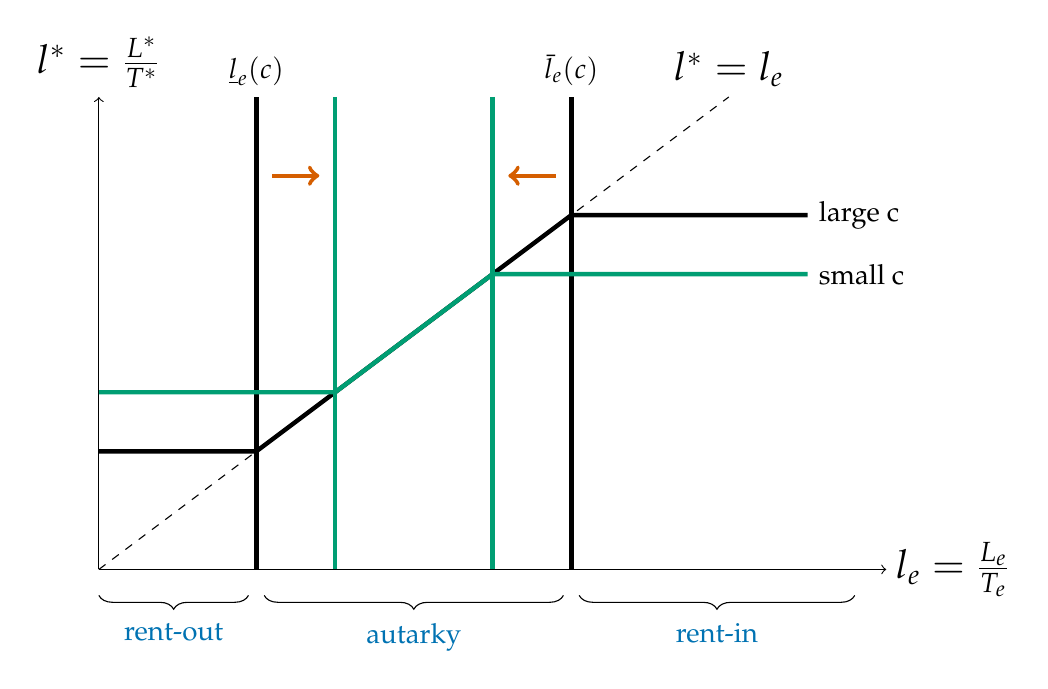
\begin{tikzpicture}
	% setup
	\draw [->] (0,0) - - (10,0) node[right]{\Large $l_e=\frac{L_e}{T_e}$};
	\draw [->] (0,0) - - (0,6) node[above]{\Large $l^*=\frac{L^*}{T^*}$};
	\draw [dashed] (0,0) -- (8, 6) node[above]{\Large $l^*=l_e$};
	% original optimization
	\draw [ultra thick] (2,0) -- (2,6) node[above]{$\underline{l}_e(c)$};
	\draw [ultra thick] (6,0) -- (6,6) node[above]{$\bar{l}_e(c)$};
	\draw [ultra thick] (0,1.5) -- (2,1.5)--(6,4.5)--(9,4.5) node[right,black]{large c} ;
	\draw [decorate,decoration={brace,amplitude=5pt,mirror,raise=2ex}] (0,0) -- (1.9,0) node[midway, below, blue, yshift=-1.6em, align=center]{rent-out};
	\draw [decorate,decoration={brace,amplitude=5pt,mirror,raise=2ex}] (2.1,0) -- (5.9,0) node[midway, below, blue, yshift=-1.6em, align=center]{autarky};
	\draw [decorate,decoration={brace,amplitude=5pt,mirror,raise=2ex}] (6.1,0) -- (9.6,0) node[midway, below, blue, yshift=-1.6em, align=center]{rent-in};
	% new optimization, change c given theta
	\onslide<2>{
	\draw [ultra thick, green] (3,6) -- (3,0);
	\draw [ultra thick, green] (5,6) -- (5,0);
	\draw [ultra thick, green] (0,2.25) -- (3,2.25)--(5,3.75)--(9,3.75) node[right, black]{small c};
	\draw [->, ultra thick, red] (2.2,5) -- (2.8, 5);
	\draw [->, ultra thick, red] (5.8,5) -- (5.2, 5);
	}
	\end{tikzpicture}}
\end{frame}




%%%%%%%%%%%%%%%%%%%%%%%%%%%%%%%%%%%
%%%%%%%%%%%%%%%%%%%%%%%%%%%%%%%%%%%
%%%%%%%%%%%%%%%%%%%%%%%%%%%%%%%%%%%
%%%%%%%%%%%%%%%%%%%%%%%%%%%%%%%%%%%
\section{Data}

%%%%%%%%%%%%%%%%%%%%%%%%%%%%%
\begin{frame}{Data}
\end{frame}



%%%%%%%%%%%%%%%%%%%%%%%%%%%%%%%%%%%
%%%%%%%%%%%%%%%%%%%%%%%%%%%%%%%%%%%
%%%%%%%%%%%%%%%%%%%%%%%%%%%%%%%%%%%
%%%%%%%%%%%%%%%%%%%%%%%%%%%%%%%%%%%
\section{Empirical Strategy \& Results}

%%%%%%%%%%%%%%%%%%%%%%%%%%%%%%%%%%%
%%%%%%%%%%%%%%%%%%%%%%%%%%%%%%%%%%%
\subsection*{Regressions on subprime lending}

%%%%%%%%%%%%%%%%%%%%%%%%%%%%%
\begin{frame}{Equations}
The baseline specification: 
\begin{equation*}
    Y_{i,t} = \underbrace{\beta_1 [ Bank_i \times \mathbbm{1}\{ t \leq 2009 \} ]}_{\text{\textcolor{red}{Null hypothesis: $\beta_1=0$}}} + \beta_2 bank_i + X_{i, 2004}' \gamma + \delta_t + \theta_s + \epsilon_{i,t}
\end{equation*}

\begin{wideitemize}
    \item <1-> $Y_{i,t}$: share of mortgages that are subprime. 
    \begin{itemize}
        \item [-] All mortgage originations.
        \item [-] ``Homogeneous'' mortgage originations: conventional, conforming, 1-4 families, first lien, owner-occupied.
    \end{itemize}
    
    \item <2-> $Bank_i$: bank dummy; $\mathbbm{1}\{ t \leq 2009 \}$: dummy of credit expansion period. 
    
    \item <3> $X_{i, 2004}'$: Covariates in year 2004 (robust to 1-year lags).
    
    \item <3> $\delta_t$ and $\theta_s$: year and state fixed effects.
\end{wideitemize}
\end{frame}

%%%%%%%%%%%%%%%%%%%%%%%%%%%%%
\begin{frame}{A table with columns showing up sequentially}
\begin{table}
\centering
\begin{adjustbox}{max width=0.75\textwidth}
\begin{tabular}{lc<{\onslide<2->}c<{\onslide<3->}cc<{\onslide}}
  \toprule
  &\multicolumn{2}{c}{Subprime Share (\%)}&\multicolumn{2}{c}{Subprime Share (\%)}\\\cmidrule(lr){2-3}\cmidrule(lr){4-5}
  &\multicolumn{1}{c}{All}&\multicolumn{1}{c}{Homogeneous}&\multicolumn{1}{c}{All}&\multicolumn{1}{c}{Homogeneous}\\
  \midrule
  bank $\times$ $\mathbbm{1}\{ Year <=2009 \}$&    7.216***&    5.456***&    7.837***&    5.064***\\
                  &  (0.439)   &  (0.593)   &  (0.441)   &  (0.579)   \\
  \addlinespace
  bank            &    7.756***&    8.727***&            &            \\
                  &  (0.998)   &  (1.247)   &            &            \\
  \addlinespace
  Institution Characteristics & $\times$   & $\times$   &            &            \\
  \addlinespace
  Borrower Characteristics & $\times$   & $\times$   & $\times$   & $\times$   \\
  \addlinespace
  State Controls  & $\times$   & $\times$   & $\times$   & $\times$   \\
  \addlinespace
  State FE        & $\times$   & $\times$   &            &            \\
  \addlinespace
  Institutional FE&            &            & $\times$   & $\times$   \\
  \addlinespace
  Year FE         & $\times$   & $\times$   & $\times$   & $\times$   \\
  \midrule
  $\mathnormal{N}$&    71228   &    63821   &    70962   &    63475   \\
  $\mathnormal{R^2}$&    0.241   &    0.306   &    0.588   &    0.617   \\
  Outcome mean    &   12.912   &   18.124   &   12.916   &   18.127   \\
  \bottomrule
  \end{tabular}
\end{adjustbox}
\end{table}
\end{frame}


%%%%%%%%%%%%%%%%%%%%%%%%%%%%%%%%%%%
\begin{frame}{A table with rows showing up sequentially}
\begin{table}[h]
\centering
\begin{adjustbox}{max width=0.75\textwidth}
\begin{threeparttable}
\begin{tabular}{l*{2}{c}}
	\toprule
	& \multicolumn{2}{c}{Average marginal effects} \\
	\midrule
	\onslide<1->{\textbf{Panel A:} & & \\
	\emph{Baseline: work off-farm locally} & \emph{stay on farm} & \emph{work off-farm outside hometown} \\
	\addlinespace
	land right intensity&     -0.0224** &      0.0175*  \\
                    &    (0.0108)   &    (0.0103)   \\
	\midrule
	}
	\onslide<2>{\textbf{Panel B:} & & \\
	\emph{Baseline: work off-farm seasonlly} & \emph{stay on farm} & \emph{work off-farm permanently} \\
	\addlinespace
	land right intensity&     -0.0173*  &      0.0084   \\
                    &    (0.0101)   &    (0.0108)   \\
	\midrule
	}
	\onslide<1->{Observations & 7678 & 7678 \\
	\bottomrule
	}
\end{tabular}				
\end{threeparttable}
\end{adjustbox}
\end{table}	
\end{frame}


%%%%%%%%%%%%%%%%%%%%%%%%%%%%%
\begin{frame}[label=robustness_check_subprime]{Robustness checks: using hyperlinks}
Results are robust to alternative methods, samples, and dependent variables.
\begin{wideitemize}
    \item <1-> Matched sample (by propensity score) \hyperlink{subprime_match}{\beamergotobutton{Results using matched sample}} 
\end{wideitemize}
\end{frame}



%%%%%%%%%%%%%%%%%%%%%%%%%%%%%%%%%%%
%%%%%%%%%%%%%%%%%%%%%%%%%%%%%%%%%%%
%%%%%%%%%%%%%%%%%%%%%%%%%%%%%%%%%%%
%%%%%%%%%%%%%%%%%%%%%%%%%%%%%%%%%%%
\section{Conclusions \& next steps}

%%%%%%%%%%%%%%%%%%%%%%%%%%%%%%%%%%%
\begin{frame}{Conclusions}
\end{frame}

\begin{frame}
\centering
\Large{Thank You!} 
\vspace{2em}

\large{Comments and suggestions \\ kangli.li@wisc.edu}
\end{frame} % to enforce entries in the table of 

%%%%%%%%%%%%%%%%%%%%%%%%%%%%%%%%%%%
\begin{frame}
\end{frame} % to enforce entries in the table of contents



%%%%%%%%%%%%%%%%%%%%%%%%%%%%%%%%%%%%%%%%%
%%%%%%%%%%%%%%%%%%%%%%%%%%%%%%%%%%%%%%%%%
%%%%%%%%%%%%%%%%%%%%%%%%%%%%%%%%%%%%%%%%%
%%%%%%%%%%%%%%%%%%%%%%%%%%%%%%%%%%%%%%%%%
\appendix 

%% subprime
%%%%%%%%%%%%%%%%%%%%%%%%%%%%%%%%%%%
\begin{frame}[label=subprime_match]{hyperlink referenced page with a retun button}
\hfill \hyperlink{robustness_check_subprime}{\beamergotobutton{Return}}
\end{frame}

\end{document}
